\section{Deep versus wide networks}

\subsection*{Subtask 1}

\footnotesize
\begin{longtable}{|m{0.5\textwidth}|m{0.43\textwidth}|} \hline
\textbf{Code Snippet} & \textbf{Description} \\ \hline
\begin{lstlisting}
import torch
import torch.nn as nn
import torch.utils.data as data
...
\end{lstlisting} & Imports of the necessary modules\\ \hline
\begin{lstlisting}
print("Using torch", torch.__version__)
device = torch.device("cuda") if torch.cuda.is_available() else torch.device("cpu")
print("Device", device)
\end{lstlisting} & Figuring out the device in order to be able to later move tensors and models to the respective device as easily as possible and ideally, in the case of a GPU, to achieve faster training and inference times. \\ \hline
\begin{lstlisting}
class XORDataset(data.Dataset):
    def __init__(self, size, std=0.1, device=device):
        super().__init__()
        self.size = size
        self.std = std
        self.generate_continuous_xor()

    def generate_continuous_xor(self):
    ...
\end{lstlisting} & Creation of the XOR data set with the parameters \lstinline|size|(= the number of data to be generated), \lstinline|std| (= the standard deviation of the noise to be added to the data set) and \lstinline|device| (= the device on which the data is to be processed). With \lstinline|torch.randint|, \lstinline|size| 2D data is generated, which can take the values 0 or 1 per component. If the sum of both components of the 2D data equals 0, then this corresponds to a true XOR statement, otherwise not. In addition, normally distributed noise is added with \lstinline|torch.randn|.  \\ \hline
\begin{lstlisting}
def visualize_binary_samples(dataset):
    (data,label) = dataset.toNumpy()
    data_0 = data[label == 0]
    data_1 = data[label == 1]

    plt.figure(figsize=(4, 4))
    ...

dataset = XORDataset(size=200)
print("Size of dataset:", len(dataset))
print("Data point 0:", dataset[0])
visualize_binary_samples(dataset)
plt.show()
\end{lstlisting} & Visualisation of 200 XOR data in a 2D representation. The x-axis corresponds to the first component of the data, the y-axis to the second component. The truth content of the XOR statement (or the label of the data) is displayed in two different colours. \\ \hline
\begin{lstlisting}
class SimpleClassifier(nn.Module):
    def __init__(self, src, tg, depth, width, device=device):
        super().__init__()
        self.enc_sizes = [src, tg, depth, width]
        functionLst = [nn.Linear(src, width), nn.Identity()]
        self.model = nn.Sequential(*functionLst)
        self.model.to(device)

    def forward(self, x):
        x = self.model(x)
        x = x.squeeze(dim=1)
        return x
\end{lstlisting} & The model of the neural network, which is created using Pytorch's \lstinline|nn.Module|. An object instance of the SimpleClassifier class is generated via constructor of the variables \lstinline|src, tg, depth, width, device|. The constructor calls the inherited \lstinline|super| constructor and creates a sequential model with a linear layer and the identity as an activation function. Since the XOR problem is not separable and therefore cannot be solved in this linear form, this model would not provide an accurate solution to the classification problem. Therefore, several layers are necessary, as the following subtasks show.

The \lstinline|forward| function performs a pass through the network. Since the network returns a tensor with shape (size(x), 1), the result is flattened to the dimension size(x).\\ \hline
\begin{lstlisting}
def train_model(model, optimizer, data_loader, loss_module, num_epochs=100):
    model.train()
    for epoch in range(num_epochs):
        for data_inputs, data_labels in data_loader:
            preds = model(data_inputs)
            loss = loss_module(preds, data_labels.float())
            optimizer.zero_grad()
            loss.backward()
            optimizer.step()
\end{lstlisting} & This is the main routine to train the model based on the given data (\lstinline|data_loader|), the defined optimizer (\lstinline|optimizer|) and the defined loss (\lstinline|loss_module|). At the beginning, the model is set to the training state, which allows the weights to be adjusted. Subsequently, \lstinline|num_epoch| times of each batch of the \lstinline|data_loader| are passed through the model and then the backpropagation is carried out with the loss and the selected optimizer.\\ \hline
\begin{lstlisting}
def eval_model(model, data_loader):
    model.eval()
    ...
    acc = true_preds / num_preds
    return acc
\end{lstlisting} & This is the method for evaluating and testing the results of a (trained) model. Based on the test data (ideally unknown for the model), a forward pass is performed by the network. As the outputs of the model specified here do not necessarily yield values between 0 and 1, this evaluation method uses a sigmoid function to map the predictions of the model to values between 0 and 1 and then rounds them to the binary values 0 and 1. These values are then compared with the labels of the data and the number of \lstinline|true_predictions| is counted. The number of true predictions divided by the total number of data in the test data set then provides the accuracy. As the weights of the model should no longer be adjusted in this case and no backward pass is performed, the model is set to \lstinline|eval| and the pass is performed using \lstinline|torch.no_grad()|.\\ \hline
\begin{lstlisting}
loss_module = nn.BCEWithLogitsLoss()
train_dataset = XORDataset(size=1000)
train_data_loader = data.DataLoader(train_dataset, batch_size=128, shuffle=True)
test_dataset = XORDataset(size=500)
test_data_loader = data.DataLoader(test_dataset, batch_size=128, shuffle=False, drop_last=False)

model = SimpleClassifier(src=2, tg=1, depth=0, width=0)
print(model)

optimizer = torch.optim.SGD(model.parameters(), lr=0.1)
train_model(model, optimizer, train_data_loader, loss_module, num_epochs=200)

acc = eval_model(model, test_data_loader)
print(acc)
\end{lstlisting} & The final script that brings together the various parts of the entire training and evaluation process.
\begin{enumerate}
    \item First, the loss is defined, which in this case is a BCEWithLogitsLoss, which stands for Binary Cross Entropy with combined sigmoid application. The sigmoid application ensures that the values of the model are between 0 and 1 and can be compared with the initial binary labels. 
    \item Two XOR data sets (test and training data) are then generated (see above for details) and prepared for use in the neural network via Pytorch's \lstinline|DataLoader|.
    \item The model is created with two input nodes and a single output node (no hidden layers). In this model, the \lstinline|depth| and \lstinline|width| do not yet play a role and are therefore initialised with the values 0. These are only used in the following subtasks.
    \item The optimizer is created as Stochastic Gradient Descent with a learning rate of 0.1.
    \item The model is trained with the data from the training data set (\lstinline|train_data_loader|), the created model (\lstinline|model|), the optimizer and the defined loss via \lstinline|num_epochs=200|.
    \item Finally, the accuracy is calculated using the defined \lstinline|eval_model| method.
\end{enumerate} \\ \hline
\end{longtable}

\normalsize

\clearpage

\subsection*{Subtask 2}

Below are the main changes to the given notebook described that allow a flexible calculation of the neural network in terms of depth and width:

\begin{enumerate}
    \item In the definition of the neural network, we use the variables \lstinline|depth| and \lstinline|width| to define the number of hidden layers and the neurons used per hidden layer. For \lstinline|depth| = 0 we have to introduce a special rule which allows us to define a network without a hidden layer as already described in the initial notebook from subtask 1. 

If \lstinline|depth| $> 0$, we define the connection between the input layer and the first hidden layer (\lstinline|src|, \lstinline|width|) and the last hidden layer (\lstinline|width|, \lstinline|tg|) and add further hidden layers if necessary. In particular, for \lstinline|depth| $> 1$, we define a fully-connected linear layer (\lstinline|width|, \lstinline|width|) for every additional hidden layer. 
\begin{lstlisting}
class SimpleClassifier(nn.Module):
    def __init__(self, src, tg, depth, width, device=device):
        if depth == 0:
            functionLst = [nn.Linear(src, tg), nn.Identity()]
        else:
            functionLst = [nn.Linear(src, width), nn.Tanh()]
            for _ in range(depth-1):
                functionLst.append(nn.Linear(width, width))
                functionLst.append(nn.Tanh())
            functionLst.append(nn.Linear(width, tg))
            functionLst.append(nn.Identity())
        self.model = nn.Sequential(*functionLst)
        ...
\end{lstlisting}
\item Further, we adapted the evaluation method so that we can track the change in loss as well as the accuracy. Similar to the calculation of the loss in the training process, we calculate the loss using the \lstinline|loss_module| variable for the entire test data set and return it together with the calculated accuracy.
\begin{lstlisting}
def eval_model(model, data_loader, loss_module):
    model.eval() 
    ...
    with torch.no_grad():
        for data_inputs, data_labels in data_loader:
            loss = loss_module(model(data_inputs), data_labels.float())
            ...
    return acc, loss
\end{lstlisting}
\item We also had to adapt the final script in order to apply the changes listed above. In particular, we introduced the variables \lstinline|depths| and \lstinline|widths|, over which we iterated and trained a model for each combination. We also introduced a variable \lstinline|reps|, which represents the number of repetitions of the training process per combination. In order to obtain an accurate statement about the behaviour of the loss (mean, standard deviation) and the accuracy, we did not use 3 iterations (as formulated in the task), but 20. 

Finally, we collected the results for each combination of \lstinline|depths| and \lstinline|widths| in a dictionary (\lstinline|accs_with_metadata|) and printed them.
\begin{lstlisting}
loss_module = nn.BCEWithLogitsLoss()
...
depths = range(4)
widths = range(1,4)
reps = 20
accs_with_metadata = []
for i, depth in enumerate(depths):
    for j, width in enumerate(widths):
        acc = 0
        losses = []
        for i in range(reps):
            model = SimpleClassifier(src=2, tg=1, depth=depth, width=width)
            ...
            acc_temp, loss_temp = eval_model(model, test_data_loader, loss_module)
            acc += acc_temp
            losses.append(loss_temp)
                        
        accs_with_metadata.append({
            'acc': acc / reps,
            'depth': depth,
            'width': width,
            'number_of_parameters': sum(p.numel() for p in model.parameters()),
            'loss_mean': np.mean(losses),
            'loss_std': np.std(losses)
        })
        
for acc in sorted(accs_with_metadata, key=lambda x: x['acc'], reverse=True):
    print(f"Depth: {acc['depth']}, Width: {acc['width']}, Number of parameters: {acc['number_of_parameters']}, Accuracy: {acc['acc']}, Loss mean: {acc['loss_mean']}, Loss std: {acc['loss_std']}")

\end{lstlisting}
\end{enumerate}

Table \ref{tab:xor} shows the final results for the XOR-problem for the different combinations of \lstinline|depth| and \lstinline|width|. The table also includes the mean and standard deviation of the loss of the 20 repetitions of each training process for each combination. Further, the amount of trainable parameters is displayed.
\begin{table}[!htb]
\centering
\begin{tabular}{|c|c|c|c|c|c|}
\hline
\textbf{Depth} & \textbf{Width} & \textbf{Parameters} & \textbf{Mean Accuracy} & \textbf{Loss mean} & \textbf{Loss std} \\ \hline
1              & 3              & 13                  & 0.9442            & 0.2292             & 0.1509            \\ \hline
2              & 3              & 25                  & 0.8184            & 0.3734             & 0.2556            \\ \hline
3              & 3              & 37                  & 0.7753            & 0.4153             & 0.2535            \\ \hline
1              & 2              & 9                   & 0.7655            & 0.4801             & 0.1197            \\ \hline
2              & 2              & 15                  & 0.7453            & 0.4455             & 0.1557            \\ \hline
3              & 2              & 21                  & 0.6994            & 0.5031             & 0.2351            \\ \hline
1              & 1              & 5                   & 0.6986            & 0.6127             & 0.0664            \\ \hline
3              & 1              & 9                   & 0.6208            & 0.6217             & 0.0951            \\ \hline
2              & 1              & 7                   & 0.5896            & 0.6433             & 0.0823            \\ \hline
0              & x              & 3                   & 0.5120            & 0.6946             & 0.0001            \\ \hline
0              & x              & 3                   & 0.5120            & 0.6946             & 0.0001            \\ \hline
0              & x              & 3                   & 0.5120            & 0.6946             & 0.0001            \\ \hline
\end{tabular}
\caption{Final results of feed forward networks for XOR-problem using different widths and depths for hidden layers of the network}
\label{tab:xor}
\end{table}

\subsection*{Subtask 3}

\textbf{Interpretations of changing depth and width}

Table \ref{tab:xor} and a visualised representation of the results in figure \ref{fig:xor} are used to explain the effects of changes to the depth and width of the feed forward network in this task.

\begin{figure}[!htb]
    \centering
    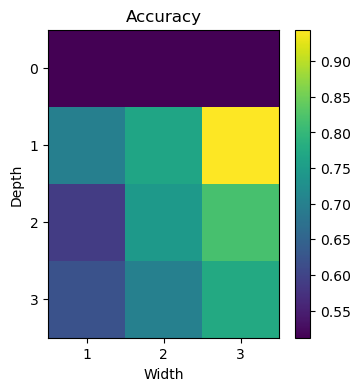
\includegraphics[width=0.4\linewidth]{Assignment_1//Report/ex_1_acc.png}
    \caption{Color map of the mean accuracy of different combinations of widths and depths for the feed forward network trying to solve the XOR problem.}
    \label{fig:xor}
\end{figure}

\begin{itemize}
    \item The XOR problem cannot be solved without a hidden layer, how the results in figure \ref{fig:xor} and table \ref{tab:xor} of \lstinline|depth| = 0 show. If \lstinline|depth| = 0, we see that the accuracy is only just over 50\% and therefore the model does not provide any information content. Drawing randomly would also provide an accuracy of 50\%. This finding proves reasonable, as the XOR problem is not linearly separable.
    \item Beyond \lstinline|depth| $>0$, if the \lstinline|depth| is increased, the accuracy seems to decrease, in particular the best results are shown in all three widths for a \lstinline|depth| of 1. This could be due to the fact that the XOR problem is fairly easy to generalise, and overfitting occurs when the complexity of the network is increased by adding additional layers.
    \item Increasing the \lstinline|width| leads to a general improvement in accuracy. Table \ref{tab:xor} and figure \ref{fig:xor} show a clear upward trend across the width. Accordingly, it can be stated that a wider network is preferable to a deeper network in this case. Only at least one hidden layer must be present, as otherwise the XOR problem cannot be solved.
\end{itemize}

\textbf{Number of Parameters for each model}

The number of parameters for each model can be found in table \ref{tab:xor}. 

\textbf{Training parameters}

\textit{
The entry in brackets after the parameter name in bold indicates the parameter actually used.}

\begin{itemize}
    \item \textbf{Training repetitions (20)}: Increasing the number of training repetitions per combination of \lstinline|depths| and \lstinline|widths| leads to a more precise evaluation of the mean value and a lower deviation of accuracy and loss for the test set. Accordingly, the statements about the resulting models become more reliable, which is why we have also increased the number of training repetitions from 3 to 20.
    \item \textbf{Training epochs (100)}: The more training epochs are carried out, the more often the model sees the training data and adapts accordingly. This can lead to the model not having sufficient opportunity to adapt to the data, particularly if the number of training epochs is too low. On the other hand, there is a risk of overfitting if the number of training epochs is too high.
    \item \textbf{Batch Size (128)}: The batch size influences after how many samples the weights of a model are adjusted. Accordingly, a higher batch size ensures larger update steps, which can potentially lead to faster convergence. On the other hand, this can also lead to overfitting of the training data. Smaller batch sizes, on the other hand, ensure a slower training process with a high probability of the model's generalisation capability.
    \item \textbf{Learning rate (0.01)}: A higher learning rate could lead to faster convergence of the model, but also harbours the risk of overshooting the desired goal. A lower learning rate, on the other hand, ensures that this does not happen, but the learning phase until the desired result is achieved takes longer. An alternative solution that incorporates the positive aspects of both sides would be an adaptive learning rate.
    \item \textbf{Optimizer (Stochastic Gradient Descent)}: As an alternative to Stochastic Gradient Descent, one could use a different optimizer, such as Adam or RMSProp. These can potentially lead to faster convergence and prevent small update steps in the optimisation process. However, they are more complex and less intuitive than the classic Stochastic Gradient Descent approach. In principle, all three variants should equally find a suitable local minimum of the model.
    \item \textit{\textbf{Loss function (Binary Cross Entropy Loss)}: The choice of loss function is not necessarily part of the training parameters, but allows nevertheless for multiple choices and therefore influences the training behaviour of a model. For example, one might use a hinge loss instead of a cross entropy loss, although the model should still be able to learn similarly well.}
    \end{itemize}

    \clearpage
    
